\documentclass[a4 paper]{article}
% Set target color model to RGB

% Portugues
\usepackage[brazilian]{babel}
\usepackage[utf8]{inputenc}
\usepackage[T1]{fontenc}


\usepackage[inner=2.0cm,outer=2.0cm,top=2.5cm,bottom=2.5cm]{geometry}
\usepackage{setspace}
\usepackage[rgb]{xcolor}
\usepackage{verbatim}
\usepackage{subcaption}
\usepackage{amsgen,amsmath,amstext,amsbsy,amsopn,tikz,amssymb,tkz-linknodes}
\usepackage{fancyhdr}
\usepackage[colorlinks=true, urlcolor=blue,  linkcolor=blue, citecolor=blue]{hyperref}
\usepackage[colorinlistoftodos]{todonotes}
\usepackage{rotating}
%\usetikzlibrary{through,backgrounds}
\hypersetup{%
pdfauthor={Ashudeep Singh},%
pdftitle={Homework},%
pdfkeywords={Tikz,latex,bootstrap,uncertaintes},%
pdfcreator={PDFLaTeX},%
pdfproducer={PDFLaTeX},%
}
%\usetikzlibrary{shadows}
% \usepackage[francais]{babel}
\usepackage{booktabs}
\newcommand{\ra}[1]{\renewcommand{\arraystretch}{#1}}

\newtheorem{thm}{Theorem}[section]
\newtheorem{prop}[thm]{Proposition}
\newtheorem{lem}[thm]{Lemma}
\newtheorem{cor}[thm]{Corollary}
\newtheorem{defn}[thm]{Definition}
\newtheorem{rem}[thm]{Remark}
\numberwithin{equation}{section}

\newcommand{\homework}[6]{
   \pagestyle{myheadings}
   \thispagestyle{plain}
   \newpage
   \setcounter{page}{1}
   \noindent
   \begin{center}
   \framebox{
      \vbox{\vspace{2mm}
    \hbox to 6.28in { {\bf GCC153:~Mineração de Dados \hfill {\small (#2)}} }
       \vspace{6mm}
       \hbox to 6.28in { {\Large \hfill #1  \hfill} }
       \vspace{6mm}
       \hbox to 6.28in { {\it Professor: {\rm #3} \hfill {\rm #4} %Name: {\rm #5}, Netid: {\rm #6}
       } }
       %\hbox to 6.28in { {\it TA: #4  \hfill #6}}
      \vspace{2mm}}
   }
   \end{center}
   \markboth{#5 -- #1}{#5 -- #1}
   \vspace*{4mm}
}

\newcommand{\problem}[2]{~\\\fbox{\textbf{Etapa #1}}\hfill (#2\%)\newline\newline}
\newcommand{\subproblem}[1]{~\newline\textbf{(#1)}}
\newcommand{\D}{\mathcal{D}}
\newcommand{\Hy}{\mathcal{H}}
\newcommand{\VS}{\textrm{VS}}
\newcommand{\solution}{~\newline\textbf{\textit{(Solution)}} }

\newcommand{\bbF}{\mathbb{F}}
\newcommand{\bbX}{\mathbb{X}}
\newcommand{\bI}{\mathbf{I}}
\newcommand{\bX}{\mathbf{X}}
\newcommand{\bY}{\mathbf{Y}}
\newcommand{\bepsilon}{\boldsymbol{\epsilon}}
\newcommand{\balpha}{\boldsymbol{\alpha}}
\newcommand{\bbeta}{\boldsymbol{\beta}}
\newcommand{\0}{\mathbf{0}}


\begin{document}
\homework{Orientações para o Projeto da Disciplina}{2019-2}{Eric Fernandes de Mello Araújo}{Versão: \today}{Student name(s)}{NetId(s)}

\textbf{Instruções importantes}: Leia todas as instruções cuidadosamente antes de começar o seu projeto e antes de submeter no Campus Virtual.
\begin{itemize}
    \item Escreva o projeto em \LaTeX. Use o modelo fornecido neste documento e inclua seu nome e sua matrícula. 
    \item Todas as etapas terão como prazo final para a entrega a meia noite do dia definido, segundo cronograma a seguir.
    \item Entregas fora do prazo acarretarão em redução de 10\% na nota para cada dia de atraso.
    \item Os projetos serão feitos individualmente.
    \item Todas as fontes consultadas deverão ser citadas.
\end{itemize}

\section*{Descrição}

O desenvolvimento da mineração de dados é reconhecidamente um dos fatores mais relevantes nas alterações das dinâmicas de comportamento no mundo nos últimos anos. O uso de técnicas de extração de informação a partir dos dados causou impactos nas áreas de marketing, política, religião e nas esferas socio-afetivas de nossa sociedade. Os resultados obtidos por meio destas técnicas têm atraído o interesse de empresas e pesquisadores para o quanto se pode aprender sobre os dados de forma automática.

Ao longo do curso, veremos as várias etapas que compõem a mineração de dados, bem como algoritmos e técnicas para este tipo de exploração. A ideia deste projeto é que seja desenvolvido um algoritmo de mineração de dados que passe por todas as etapas do processo, conforme demonstrado na figura \ref{figs:etapas}.

\begin{figure}[htb!]
    \centering
    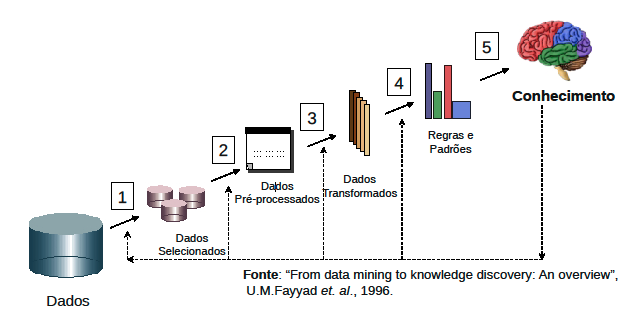
\includegraphics[width=\textwidth]{imgs/etapas_md.png}
    \caption{``From data mining to knowledge discovery: An overview'', U.M.Fayyad et. al., 1996.}
    \label{figs:etapas}
\end{figure}

As seções seguintes apresentarão as etapas do projeto, as instruções, prazos e requerimentos para a avaliação. O projeto é composto de 3 (três) etapas, 2 (duas) revisões bibliográficas e 3 (três) apresentações. O cronograma completo pode ser visto na tabela \ref{tab:crono}.

% Please add the following required packages to your document preamble:
% \usepackage{graphicx}
\begin{table}[htb!]
\centering
\resizebox{\textwidth}{!}{%
\begin{tabular}{|l|l|c|}
\hline
\textbf{Atividade} & \textbf{Descrição curta} & \textbf{Data de entrega} \\ \hline
Etapa 1 & Definição do problema a ser abordado e plano de coleta dos dados. & 09/09/2019 \\ \hline
Etapa 2 & Seleção, pré-processamento e transformação dos dados. & 21/10/2019 \\ \hline
Etapa 3 & Regras e padrões extraídos dos dados e análise do conhecimento. & 29/11/2019 \\ \hline
Revisão bibliográfica 1 & Leitura e escrita de revisão bibliográfica de 5 artigos básicos. & 27/09/2019 \\ \hline
Revisão bibliográfica 2 & Leitura e escrita de revisão bibliográfica entre 5 e 10 novos artigos relacionados com o trabalho desenvolvido. & 11/10/2019 \\ \hline
Apresentações & Apresentações dos resultados obtidos nas etapas do projeto. & Plano de curso \\ \hline
\end{tabular}%
}
\caption{Prazos para entrega das atividades a serem desenvolvidas.}
\label{tab:crono}
\end{table}


\problem{1: Definição do problema e coleta dos dados}{10}

Cada projeto deverá explorar um problema diferente que possa ser resolvido utilizando as técnicas ensinadas no curso. Para auxiliar na definição dos problemas, segue uma lista de tópicos que podem ser abordados no curso:





\subproblem{a} Write your solution here

\subproblem{b} 

\subproblem{c} 

\subproblem{d} 

% Comment: In the objective, we wrote ``Practice writing proofs'' but this is rather simple and not very rigorous?

\newpage
\problem{2: Decision Trees, Overfitting}{5+5+10+5+10+10=45}

\subproblem{a}

\subproblem{b} 

\subproblem{c}

\subproblem{d} 

\includegraphics[width=0.5\textwidth]{example-image-a}

\subproblem{e} 

\includegraphics[width=0.5\textwidth]{example-image-b}

\subproblem{f}

\includegraphics[width=0.5\textwidth]{example-image-c}

\newpage
\problem{3: Hypothesis Testing}{15+10=25}
\subproblem{a}

\subproblem{b}
\end{document} 
